\documentclass[border=10pt]{standalone}
% Shared style for the EMONI diagrams. Build: tectonic <file>.tex, then pdftocairo -svg.
\usepackage{fontspec}
\setmainfont{FiraSans}[Extension=.otf,UprightFont=*-Regular,BoldFont=*-SemiBold,ItalicFont=*-Italic,BoldItalicFont=*-SemiBoldItalic]
\setmonofont{FiraMono}[Extension=.otf,UprightFont=*-Regular,BoldFont=*-Medium,Scale=0.9]
\usepackage{tikz}
\usetikzlibrary{arrows.meta,positioning,shapes.geometric,shapes.misc,calc,fit,backgrounds}
\definecolor{eg}{HTML}{11903B}   % EMONI green
\definecolor{egl}{HTML}{E8F7EE}
\definecolor{eb}{HTML}{2A78D6}   % blue
\definecolor{ebl}{HTML}{EAF2FC}
\definecolor{eo}{HTML}{D9631E}   % orange
\definecolor{eol}{HTML}{FDF0E7}
\definecolor{ep}{HTML}{7C4DCC}   % purple
\definecolor{epl}{HTML}{F2ECFB}
\definecolor{er}{HTML}{C5221F}   % red
\definecolor{erl}{HTML}{FCEAEA}
\definecolor{ink}{HTML}{1F2328}
\definecolor{mute}{HTML}{59636E}
\definecolor{line}{HTML}{D0D7DE}
\tikzset{
  every node/.style={text=ink,font=\small},
  >={Stealth[length=2.4mm]},
  % sequence diagrams
  life/.style={draw=line,dashed,thick},
  head/.style={draw=#1,fill=#1!8,rounded corners=3pt,minimum width=27mm,minimum height=11mm,align=center,font=\small\bfseries,thick},
  act/.style={draw=#1,fill=#1!18,minimum width=2.2mm},
  msg/.style={->,thick,draw=ink},
  ret/.style={->,dashed,draw=mute},
  mlabel/.style={font=\footnotesize,fill=white,inner sep=1.5pt,align=center},
  note/.style={draw=#1,fill=#1!8,rounded corners=2pt,font=\footnotesize,align=left,inner sep=4pt},
  frag/.style={draw=mute,rounded corners=2pt},
  fraglabel/.style={draw=mute,fill=white,font=\footnotesize\bfseries,inner sep=2.5pt,anchor=north west},
  % activity diagrams
  start/.style={circle,fill=ink,minimum size=4mm,inner sep=0},
  stop/.style={circle,draw=ink,thick,minimum size=5mm,inner sep=0,path picture={\fill[ink] (path picture bounding box.center) circle (1.4mm);}},
  step/.style={draw=#1,fill=#1!8,rounded corners=5pt,thick,minimum height=9mm,minimum width=40mm,align=center,font=\small},
  step/.default=eg,
  dec/.style={diamond,aspect=2.2,draw=ink,fill=white,thick,inner sep=1.5pt,align=center,font=\footnotesize},
  flow/.style={->,thick,draw=ink},
  guard/.style={font=\footnotesize\itshape,text=mute,fill=white,inner sep=1.5pt},
  lane/.style={draw=line,fill=#1,rounded corners=4pt},
  lanetitle/.style={font=\small\bfseries,text=mute},
}

% Sequence: changing a device in the field from the dashboard (class A downlink).
\begin{document}
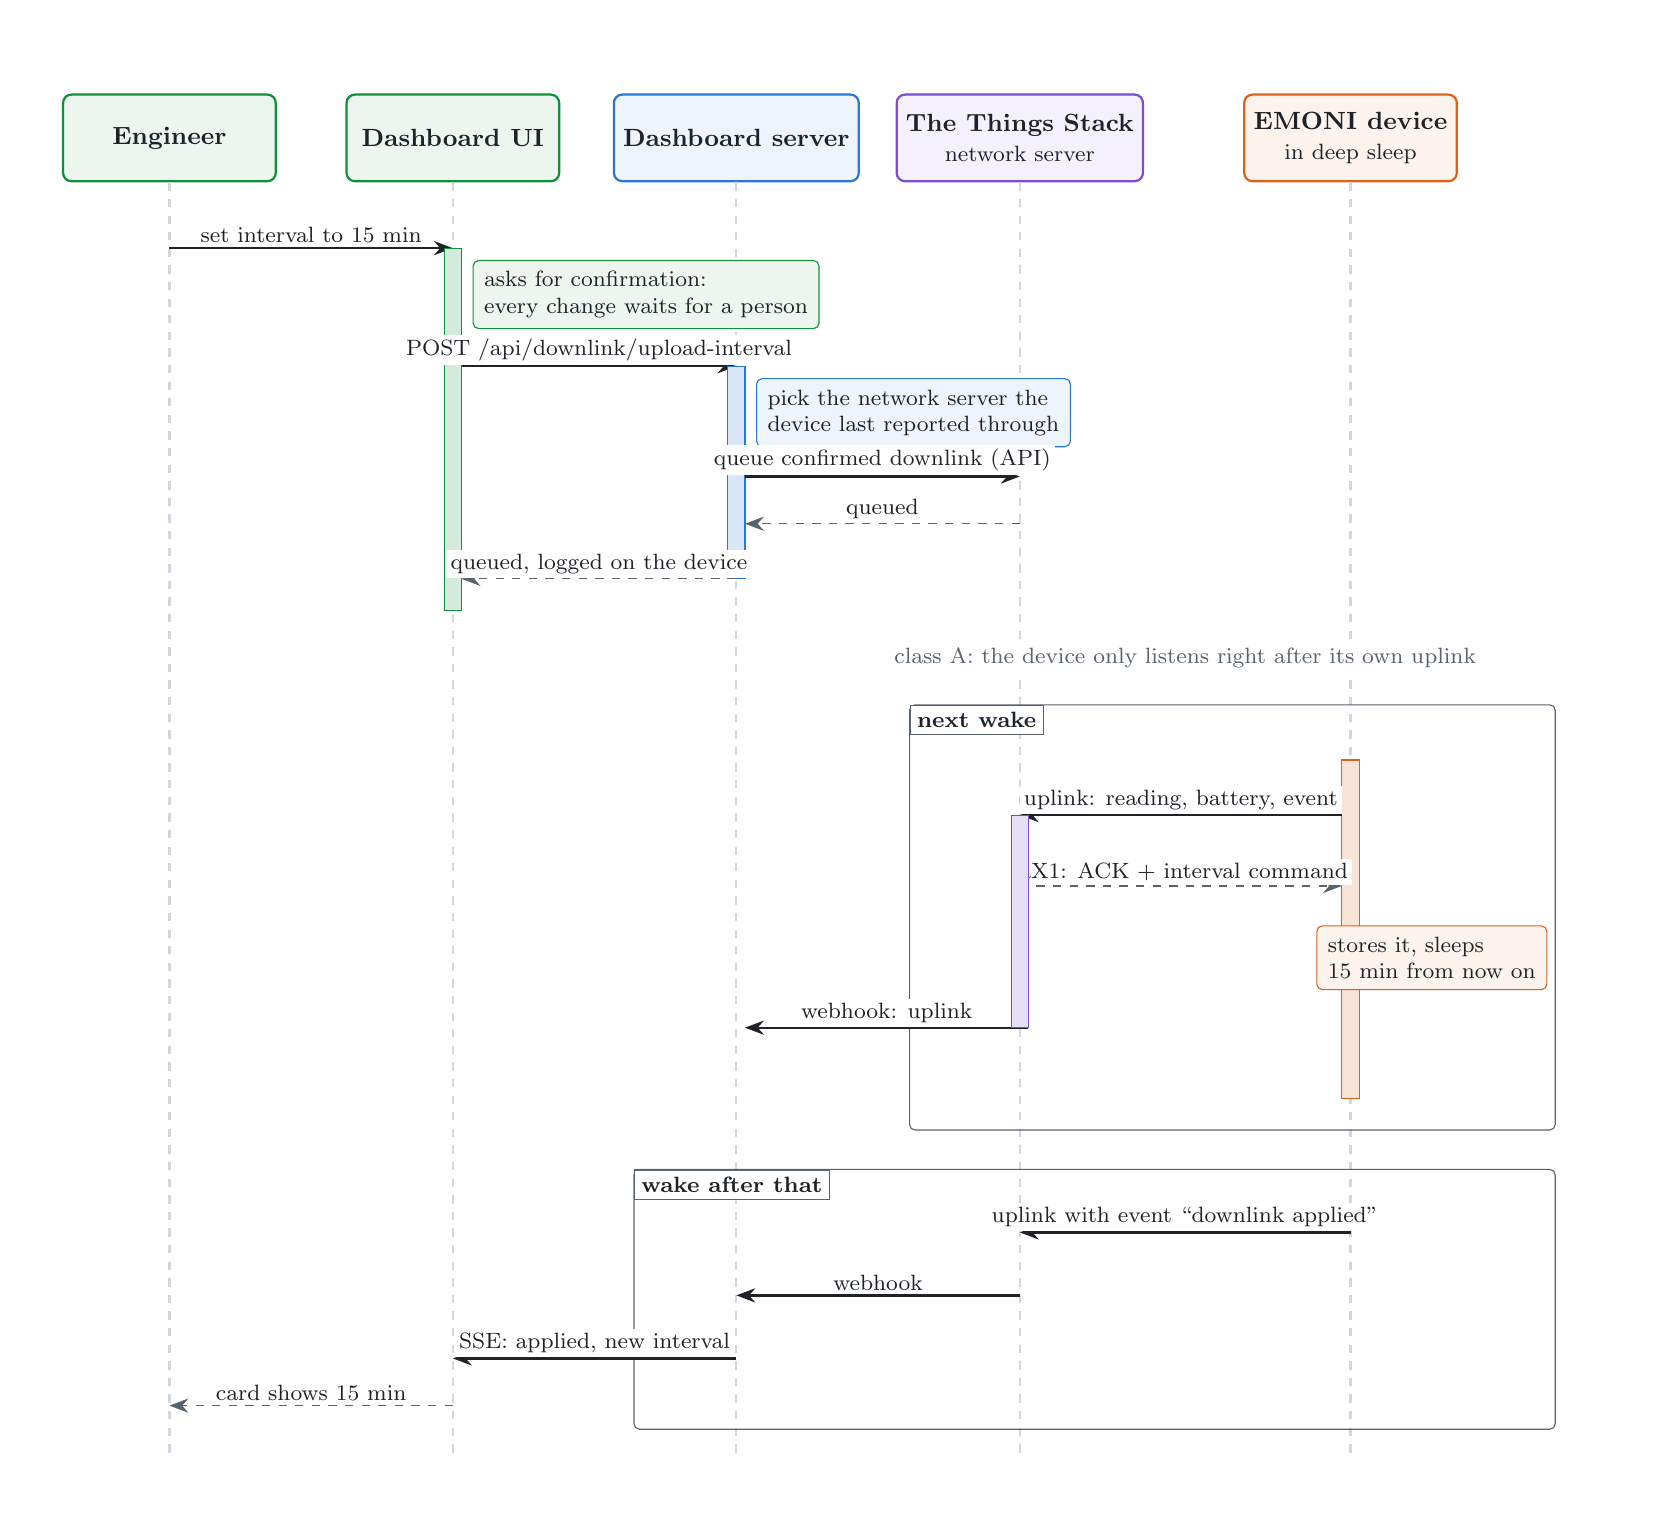
\begin{tikzpicture}[x=1cm,y=1cm]
\fill[white] (-1.8,1.4) rectangle (18.6,-17.4);
\def\B{-16.8}
\foreach \x/\n/\c/\t in {0/eng/eg/Engineer,
                         3.6/ui/eg/Dashboard UI,
                         7.2/srv/eb/Dashboard server,
                         10.8/ns/ep/The Things Stack\\{\footnotesize\mdseries network server},
                         15.0/dev/eo/EMONI device\\{\footnotesize\mdseries in deep sleep}}{
  \node[head=\c] (\n) at (\x,0) {\t};
  \draw[life] (\n.south) -- (\x,\B);
}
\draw[msg] (0,-1.4) -- node[mlabel,above]{set interval to 15 min} (3.6,-1.4);
\draw[act=eg] (3.49,-1.4) rectangle (3.71,-6.0);
\node[note=eg,anchor=north west] at (3.85,-1.55) {asks for confirmation:\\every change waits for a person};
\draw[msg] (3.71,-2.9) -- node[mlabel,above]{POST /api/downlink/upload-interval} (7.2,-2.9);
\draw[act=eb] (7.09,-2.9) rectangle (7.31,-5.6);
\node[note=eb,anchor=north west] at (7.45,-3.05) {pick the network server the\\device last reported through};
\draw[msg] (7.31,-4.3) -- node[mlabel,above]{queue confirmed downlink (API)} (10.8,-4.3);
\draw[ret] (10.8,-4.9) -- node[mlabel,above]{queued} (7.31,-4.9);
\draw[ret] (7.2,-5.6) -- node[mlabel,above]{queued, logged on the device} (3.71,-5.6);
\node[mlabel,text=mute] at (12.9,-6.6) {class A: the device only listens right after its own uplink};
% next wake
\draw[frag] (9.4,-7.2) rectangle (17.6,-12.6);
\node[fraglabel] at (9.4,-7.2) {next wake};
\draw[act=eo] (14.89,-7.9) rectangle (15.11,-12.2);
\draw[msg] (14.89,-8.6) -- node[mlabel,above]{uplink: reading, battery, event} (10.8,-8.6);
\draw[ret] (10.8,-9.5) -- node[mlabel,above]{RX1: ACK + interval command} (14.89,-9.5);
\node[note=eo,anchor=north east] at (17.5,-10.0) {stores it, sleeps\\15 min from now on};
\draw[msg] (10.91,-11.3) -- node[mlabel,above]{webhook: uplink} (7.31,-11.3);
\draw[act=ep] (10.69,-8.6) rectangle (10.91,-11.3);
% following wake
\draw[frag] (5.9,-13.1) rectangle (17.6,-16.4);
\node[fraglabel] at (5.9,-13.1) {wake after that};
\draw[msg] (15,-13.9) -- node[mlabel,above]{uplink with event ``downlink applied''} (10.8,-13.9);
\draw[msg] (10.8,-14.7) -- node[mlabel,above]{webhook} (7.2,-14.7);
\draw[msg] (7.2,-15.5) -- node[mlabel,above]{SSE: applied, new interval} (3.6,-15.5);
\draw[ret] (3.6,-16.1) -- node[mlabel,above]{card shows 15 min} (0,-16.1);
\end{tikzpicture}
\end{document}
